\section{Introduction}
\label{sec:introduction}

Chromatic localization separates stable homotopy theory into heights.
The fracture square relates height \(n\) to the lower heights through
the overlap
\[
 X_{n,p}=L_{n-1}L_{K(n)}S_p^\wedge.
\]
Here \(K(n)\) is Morava \(K\)-theory, \(L_{K(n)}\) is its localization,
and \(L_r=L_{E(r)}\) is localization at Johnson--Wilson theory;
\(L_0\) is rationalization. Describing this overlap requires both its
pieces and the maps that attach them.

We prove a filtered form of chromatic splitting in the range
\(p>n+1\). The cofibers are the sphere localizations in the classical
strong splitting list, but their extensions are retained. The map
from the first stage to \(X_{n,p}\) is the canonical localization unit.
The proof constructs
one family of product maps before applying any lower-height test.

\subsection{The theorem}

Put \(S=S_p^\wedge\) and \(D=L_{K(n)}S\). For a finite set \(I\) of
positive integers, write
\[
 d(I)=\sum_{i\in I}(2i-1),\qquad d(\varnothing)=0.
\]
All filtrations below are in the category of \(E(n-1)\)-local
\(S\)-modules; equivalences and localizations are detected on the
underlying spectra.

\begin{theorem}\label{thm:main}
Let \(n\geq1\) and let \(p>n+1\) be prime. There exist an
enumeration \(I_1,\ldots,I_{2^n}\) of the subsets of
\(\{1,\ldots,n\}\), a filtration \(F_\bullet\), and a family of
classes \(y_i\in\pi_{1-2i}D\), \(1\leq i\leq n\), with the
following properties.
\begin{enumerate}[label=(\alph*)]
\item \textbf{Filtration and unit.}
The enumeration has \(I_1=\varnothing\) and \(\max I_j\)
nondecreasing for \(j\geq2\). The filtration is
\[
 0=F_0\longrightarrow F_1\longrightarrow\cdots
 \longrightarrow F_{2^n}\xrightarrow{\simeq}X_{n,p}
\]
with \(\operatorname{cofib}(F_{j-1}\to F_j)\simeq C_{I_j}\), where
\begin{equation}\label{eq:pieces}
 \begin{aligned}
 C_\varnothing&=L_{n-1}S,\\
 C_I&=\Sigma^{-d(I)}L_{n-\max I}S
       \quad(I\ne\varnothing).
 \end{aligned}
\end{equation}
Under \(F_1=C_\varnothing\), the composite \(F_1\to X_{n,p}\) is the
canonical localization unit.
\item \textbf{Simultaneous product bases.}
For this one family, set \(y_\varnothing=1\) and
\(y_I=y_{i_1}\cdots y_{i_r}\) for \(I=\{i_1<\cdots<i_r\}\).
For every \(1\leq t<n\), the specified map
\begin{equation}\label{eq:height-basis}
 L_{K(t)}
 \left(\bigvee_{I\subseteq\{1,\ldots,n-t\}}
       \Sigma^{-d(I)}S\xrightarrow{(y_I)}D\right)
 \quad\text{is an equivalence}.
\end{equation}
\end{enumerate}
\end{theorem}

The product bases are the input to the filtration criterion of
Proposition~\ref{prop:assembly}. Its construction removes the pieces
in blocks of decreasing chromatic height. For \(n>1\), the first block
consists of the unit and the degree-\(-1\) piece, both localized at
\(E(n-1)\). For \(2\leq j<n\), the block with \(\max I=j\)
has \(2^{j-1}\) pieces; after removing it, the remaining quotient
has height at most \(n-j-1\). The last quotient is rational, and its
\(2^{n-1}\) pieces are chosen from rational dimensions. Those last
pieces are not identified with the products \(y_I\) containing \(n\).

The resulting filtration retains the attaching maps. Thus the theorem
answers the ordered-filtration formulation studied here; it does not
assert the classical wedge decomposition or a retraction of the unit.
We make no sharpness claim for the prime bound.

At height one the two cofibers are \(H\Qp\) and
\(\Sigma^{-1}H\Qp\). At height three, where the range is \(p\geq5\),
one permitted order is
\[
\begin{gathered}
 L_2S,\quad\Sigma^{-1}L_2S,\quad
 \Sigma^{-3}L_1S,\quad\Sigma^{-4}L_1S,\\
 \Sigma^{-5}H\Qp,\quad\Sigma^{-6}H\Qp,\quad
 \Sigma^{-8}H\Qp,\quad\Sigma^{-9}H\Qp.
\end{gathered}
\]
\subsection{Proof strategy}
\label{intro:strategy}

Two issues separate the desired product bases from a calculation of
cohomological ranks. The cohomology generators must be represented by
sphere classes, and those representatives must induce the required
basis under every lower-height test. The proof develops these two
inputs separately and compares their actual actions before applying
the tests. Figure~\ref{fig:proof-architecture} shows where they meet.

For the coefficient input, fix \(1\leq t<n\), put \(m=n-t\), and
choose a finite field \(k\) containing the Honda fields in use, with
degree prime to \(p\). The characteristic-\(p\) deformation stratum
has rings
\[
A_t=k[[x_t,\ldots,x_{n-1}]],\qquad B_t=A_t[1/x_t].
\]
Let \(\mathcal B_{n,t}\) be the algebraic union of finite covers of
\(B_t\) that mark the connected height-\(t\) formal group, leaving
its \'etale Tate module unmarked. A cochain on a compact source uses
one finite cover and one common pole bound. Write \(P_n\) for the
ordinary height-\(n\) stabilizer, the unit group of the maximal order
in the division algebra over \(\Qp\) of invariant \(1/n\).

Sections~\ref{sec:rings}--\ref{sec:support} compare these algebraic
coefficients with integral compact supports. Finite covers that mark
both the connected group and its \'etale basis carry translation
torsors. Their normalized transfers have a concrete feature: in
invariant-volume coordinates, the transpose is the actual Frobenius
on finite-cover functions. The perfected frame quotient is a space
of independent bundle extensions. Its compact supports, computed by
a rational flag resolution, give a finite stable transfer image.

The passage from that stable image to coefficient finiteness is a
three-part induction, organized in
Theorem~\ref{thm:coefficient-finiteness}. Section~\ref{sec:compact}
proves compact finiteness using a fixed translation extension
operation. Section~\ref{sec:boundary} removes the pole bound by
retaining the nilpotent transverse deformation at each boundary
stratum. Section~\ref{full:section} then passes to the full frame
tower and proves the individual-row norm-character filtrations
needed at later boundary steps. The order on \((n,n-t)\) makes these
dependencies inductive: a boundary step uses full-frame rows at
larger starting height and compact coefficients at smaller total
height. Throughout, the constant \(P_n\)-cochain action is retained.

The second input is one family of stable constants.
Sections~\ref{sec:constants}--\ref{sec:generators} construct
\[
u_i\in\pi_{1-2i}C^*_{\mathrm{cts}}(P_n;S),\qquad 1\leq i\leq n,
\]
where the coefficient sphere has trivial \(P_n\)-action. A common
modification space compares division and matrix constant cochains;
on the extension space, it identifies the action with upper-left
matrix-block restriction. Integral regulator and top-volume
calculations normalize the classes so that their mod-\(p\) Hurewicz
images have nonzero exterior product. Write
\(\xi_i\in H^{2i-1}_{\mathrm{cts}}(P_n;k)\) for these images
under \(S\to H\Fp\), followed by scalar extension to \(k\).

Section~\ref{full:module-section} brings the two inputs together.
A parabolic weight calculation and a natural top-edge map identify
the coefficient module with the regular exterior module for the
specified classes. Its degree-zero generator is the coefficient unit:
Proposition~\ref{prop:constant-module} proves
\[
\bigwedge_k(e_1,\ldots,e_m)
\xrightarrow{\;\sim\;}H^*_{\mathrm{cts}}(P_n;\mathcal B_{n,t}),
\qquad e_i\longmapsto\xi_i\cdot1,\quad |e_i|=2i-1.
\]
The same rank-\(n\) family supplies this map for every \(t\).

Finally, Section~\ref{sec:spectral} applies ordinary residue smash
to the completed Morava descent resolution. Flatness and finite
algebraic base change recover the coefficient complex above,
including its semilinear first coface. The classes \(u_i\) map to
the classes \(y_i\) in \(D\); their products give compatible lifts
of every basis vector through the totalization tower. Consequently
the associated-graded basis is realized by the specified maps in
\eqref{eq:height-basis}. Section~\ref{sec:assembly} proves in advance
the final step: successive cofibers lower the height of the quotient,
rational independence determines its last block, and finite pullbacks
produce the filtration with its prescribed unit.

\begin{figure}[htbp]
\centering
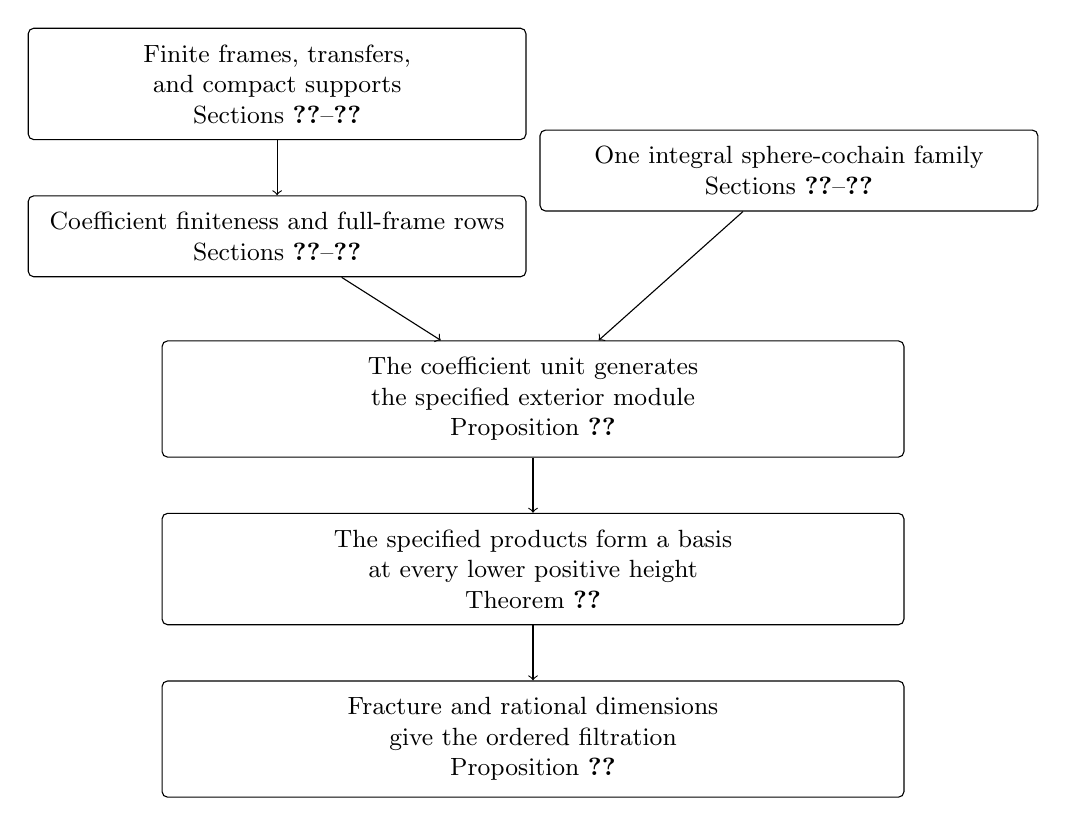
\begin{tikzpicture}[
  every node/.style={align=center,font=\small},
  box/.style={draw,rounded corners=2pt,inner sep=6pt,text width=5.9cm}
]
\node[box] (geometry) at (-3.25,0)
  {Finite frames, transfers, and compact supports\\
   Sections~\ref{sec:rings}--\ref{sec:support}};
\node[box,anchor=north] (finiteness)
  at ([yshift=-7mm]geometry.south)
  {Coefficient finiteness and full-frame rows\\
   Sections~\ref{sec:compact}--\ref{full:section}};
\node[box] (classes) at (3.25,-1.1)
  {One integral sphere-cochain family\\
   Sections~\ref{sec:constants}--\ref{sec:generators}};
\node[box,text width=9cm,anchor=north] (module)
  at ([xshift=3.25cm,yshift=-8mm]finiteness.south)
  {The coefficient unit generates\\the specified exterior module\\
   Proposition~\ref{prop:constant-module}};
\node[box,text width=9cm,anchor=north] (bases)
  at ([yshift=-7mm]module.south)
  {The specified products form a basis\\at every lower positive height\\
   Theorem~\ref{thm:height-bases}};
\node[box,text width=9cm,anchor=north] (filtration)
  at ([yshift=-7mm]bases.south)
  {Fracture and rational dimensions\\give the ordered filtration\\
   Proposition~\ref{prop:assembly}};
\draw[->] (geometry) -- (finiteness);
\draw[->] (finiteness) -- (module);
\draw[->] (classes) -- (module);
\draw[->] (module) -- (bases);
\draw[->] (bases) -- (filtration);
\end{tikzpicture}
\caption{The two inputs to the prescribed product bases. The left
branch keeps the algebraic coefficient topology and its constant-cochain
action; the right constructs the classes that act. Ordinary residue
descent recognizes their products, and the independent rational
calculation supplies the last filtration block.}
\label{fig:proof-architecture}
\end{figure}

\subsection{History and the ingredients of the proof}

Hopkins' chromatic splitting conjecture, recorded by Hovey
\cite[Conjecture~4.2]{Hovey}, proposes classes, factorizations, and a
splitting of a canonical cofiber sequence. Its weak consequence asks
for a retraction of the canonical unit comparison \cite[p.~2]{Hovey}. Barthel and
Beaudry review a revised strong formulation
\cite[Conjecture~6.3 and Remark~6.4]{BB}. The exterior-indexed
summand pattern motivates \eqref{eq:pieces}; Theorem~\ref{thm:main}
realizes that pattern as the successive cofibers of an ordered filtration
in the stated prime range.

Hovey's July 1993 account records the height-one case and the
height-two case at \(p>3\) as known, attributing the latter to Hopkins using
Shimomura--Yabe \cite[pp.~17--19]{Hovey}. Goerss--Henn--Mahowald
prove the height-two splitting at \(p=3\)
\cite[Theorem~1.2]{GHM2014}. At height two and prime two, Beaudry
disproved the original strong formula
\cite[Theorem~1.4]{Beaudry2017}. Beaudry--Goerss--Henn's
corrected calculation has additional Moore-spectrum terms and retains
a split unit \cite[Theorem~1.1.6]{BGH2022}.

Barthel--Schlank--Stapleton--Weinstein determine the rational
homotopy of the \(K(n)\)-local sphere at every positive height and
prime \cite[Theorem~A]{BSSW}. Their result gives
\begin{equation}\label{eq:rational-dimensions}
 \dim_{\Qp}\pi_{-b}L_0D
  =\#\{I\subseteq\{1,\ldots,n\}:d(I)=b\}.
\end{equation}
This determines the size of the last, rational block. It does not
identify the maps in \eqref{eq:height-basis}. We do not identify its
individual rational generators with our integral \(y_i\).

Torii developed common-coefficient comparisons between adjacent
Morava theories and the localized descent spectral sequences they
induce, including the unit comparison and survival of the reduced-norm
class \cite[Theorems~4.7, 6.2, 7.6, and~8.1]{ToriiTranschromatic}.
The characteristic-\(p\) period domains of
Barthel--Mann--Ray--Schlank--Senger--Weinstein--Zhou provide a geometric
approach to the coheight-one problem. For \(n\geq2\), their
Corollary~B shows that the map
\[
L_{K(n-1)}S\ \vee\ \Sigma^{-1}L_{K(n-1)}S
       \longrightarrow L_{K(n-1)}D
\]
represented by the unit and the Devinatz--Hopkins class admits a
retraction when \((p-1)\nmid(n-1)\). Their Theorem~C gives the
full equivalence at height two and odd primes \cite{BMR}.
Their relative two-tower description also identifies the determinant
normalization for positive-height strata
\cite[Theorems~2.0.1 and~2.6.3]{BMR}.

The coefficient distinction emphasized in \cite[Section~1.5]{BMR}
is essential here. At intermediate heights \(0<t<n-1\), analytic
functions on the punctured stratum form a larger ring than the
arithmetic coefficients arising from ordinary chromatic base change.
Our height test requires the algebraic union
\(\mathcal B_{n,t}\) with its common finite-stage and bounded-pole
cochains. Sections~\ref{sec:support}--\ref{full:section} connect its
cohomology to integral compact supports through transfer and the
boundary induction, while retaining that algebraic coefficient
convention.

To connect the finite frame tower to integral compact supports, we
pass from torsion coordinates to bundle extensions and track the transfer
system. Hopkins and Gross relate the rigid generic Lubin--Tate deformation
space to projective geometry through an equivariant period map
\cite[Theorem~1]{HopkinsGross1994}.
The finite torsion-coordinate calculation is closely related to
Strauch's analysis of universal formal modules \cite{Strauch};
the exact-height connected markings use the formal-group
classification in \cite[Lecture~14, Theorem~1]{LurieFormalGroups}.
The passage to bundles uses the Fargues--Fontaine curve
\cite{FarguesFontaine}, the universal-cover description of
Scholze--Weinstein \cite{ScholzeWeinstein}, the relative slope
classification of Fargues--Scholze \cite{FarguesScholze}, and the
full faithfulness for positive section sheaves of
Ansch\"utz--Le Bras \cite{AnschuetzLeBrasFourier}. Primitive comparison
and open--closed localization for integral coefficients supply the
geometric comparisons \cite{ScholzeHodge,PignonYwanne}.
The compact-parameter and incidence arguments in
Section~\ref{sec:support} establish the uniformity required to apply
these comparisons to the finite marking tower and its transfers.

To obtain one family of acting sphere classes, we compare constant
cochains and construct stable representatives with integral product
normalization. Dotto--Le Hung compute the required mod-\(p\) constant
cohomology in the range \(a<p-1\) \cite{DLH}; the integral deduction
is included in Section~\ref{sec:constants}. The same section uses
the integral Drinfeld-space calculation of
Colmez--Dospinescu--Nizio\l\ \cite{CDN} to compare constant cochains
through a common modification space. The construction of stable
representatives then uses the continuity theorem of
Geisser--Hesselholt \cite{GeisserHesselholt}, in the modern formulation
of Clausen--Mathew--Morrow \cite{CMM}, the local cyclotomic-trace
comparison of Hesselholt--Madsen \cite{HesselholtMadsenWitt}, and the
chosen coordinates in topological cyclic homology of
Blumberg--Mandell \cite{BlumbergMandellTC}. The regulator comparison of Huber--Kings
\cite{HuberKings} and the suspended-Chern volume calculation of
Huber--Soergel \cite{HuberSoergel} supply the rational normalization
data. Section~\ref{sec:generators} combines them with local lattice and
sphere-lifting arguments to obtain the integral normalization needed
for the products to remain generators modulo \(p\).
